% !TeX root = ../tesis.tex

\textbf{Falta emplear las relacinoes de ortogonalidad para calcular las secciones de extincion y edmás}
\clearpage


In Fig. \ref{fig:Mieefficiencies} the extinction  $Q_\text{ext}$ and the scattering  $Q_\text{sca}$ efficiencies of a 12.5 nm AuNP are shown as function of the wavelength $\lambda$ of the incident planewave illuminating the NP. Two matrices were considered in Fig. \ref{fig:Mieefficiencies}: a matrix with a refractive index $n_\text{mat} = 1$ (black lines) modelling air and a matrix with a refractive index $n_\text{mat} = 1.33$ (orange lines) modelling water in the visible spectrum ( $450\text{ nm} < \lambda < 750 \text{ nm}$).  The experimental dielectric function for Au reported by \citeauthor{johnson_optical_1972} \cite{johnson_optical_1972}  was employed to model the electromagnetic response of the spherical AuNP nevertheless, this data corresponds to a bulk sample, meaning that it may not reproduce the optical behavior of a NP since surface effects cease to be neglectable  due to their spacial dimensions \cite{noguez_surface_2007}.   In order to study  the optical properties of AuNP while considering  surface effects,  a size correction to the dielectric function was performed as described in Appendix \ref{app:SizeCorrection}. The efficiencies of the 12.5 nm AuNP  taking into account a dielectric function with (dashed lines) and without (solid lines) a size correction were compared for both considered matrices; on each curve the wavelength of their maximum value, which corresponds to the wavelength of the LSPR, is indicated.


 \begin{figure}[h!]
 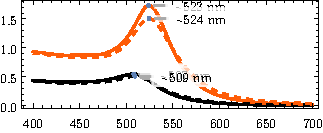
\includegraphics[scale=1.4]{1-Theory-Figs/Mie-Au/extinction-12--5nm-Au-in-H2O.pdf}
 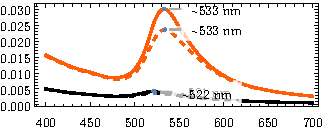
\includegraphics[scale=1.4]{1-Theory-Figs/Mie-Au/scattering-12--5nm-Au-in-H2O.pdf}
\caption[Extinction and Scattering Corss Section of a 12.5 nm Au spherical NP embeded into a vacuum- and into a waterlike environment]{ \textbf{a)} Extinction $Q_\text{ext}$ and \textbf{b)} Scattering $Q_\text{sca}$ a Efficiencies of a 12.5 nm Au spherical NP embeded into a vacuum-like matrix (black, $n_\text{mat} = 1$)  and into a water-like matrix (orange, $n_\text{mat} = 1.33$), as function of  the wavelength $\lambda$ of the incident plane wave.  The solid curves were calculated by considering no size effects on the dielectric function of the AuNP, while the dashed curves considers a size correction to it; the experimental data of \citeauthor{johnson_optical_1972} \cite{johnson_optical_1972} was employed.} 
\label{fig:Mieefficiencies} 
 \end{figure}
 
From the extinction and scattering efficiencies in Fig. \ref{fig:Mieefficiencies}, two main spectral tendencies arises between these quantities: on the overall value of the efficiencies and on the spectral position of their maximum. Since the scattering efficiency is two orders of magnitude smaller than the extinction efficiency within the visible range, the main energy loss mechanism is absorption, as stated by the Optical Theorem [Eq. \eqref{eq:Cext}]. Even though the 12.5 nm AuNP absorbs more light than what it scatters, both phenomena are present. For example, when the  studied AuNP is embedded in air, the wavelengths at which it absorbs and scatters the most are $\sim 509$ nm and $\sim 522$ nm, respectively. When the AuNP is embedded into water, the absorption of light is optimized at a wavelength of $\sim 525$ nm, while the scattering is optimized at $\sim 533$ nm. For both an air and a water matrix, the wavelength of most scattering is $\sim 10$ nm redshifted relative to the wavelength of most absorption. As it can be seen, the extinction and scattering may have different spectral tendencies as already discussed, yet they share common characteristics   when the dependency on the embedding media or on the size of the particle are studied.

The scattering and the absorption efficiencies of a 12.5 nm AuNP present an overall increase within the visible range when the refractive index of the matrix, the embedding media,  increases. This can be seen by comparing the black curves ($n_\text{mat} = 1$) with the orange curves ($n_\text{mat} = 1.33$), which are at least 
 

 
 
 
 \begin{figure}
 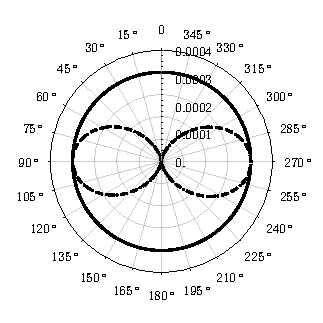
\includegraphics[scale=1]{1-Theory-Figs/Mie-Au/S-12--5nm-Au-in-Air.pdf}
 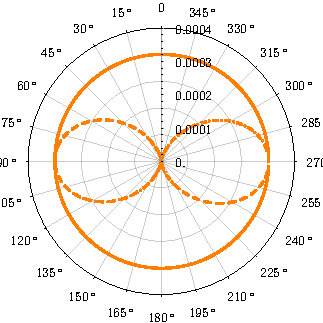
\includegraphics[scale=1]{1-Theory-Figs/Mie-Au/S-12--5nm-Au-in-H2O.pdf}
\caption[Extinction and Scattering Corss Section of a 12.5 nm Au spherical NP embeded into a vacuum- and into a waterlike environment]{ \textbf{a)} Extinction $Q_\text{ext}$ and \textbf{b)} Scattering $Q_\text{sca}$ a Efficiencies of a 12.5 nm Au spherical NP embeded into a vacuum-like matrix (black, $n_\text{mat} = 1$)  and into a water-like matrix (orange, $n_\text{mat} = 1.33$), as function of  the wavelength $\lambda$ of the incident plane wave.  The solid curves were calculated by considering no size effects on the dielectric function of the AuNP, while the dashed curves considers a size correction to it; the experimental data of \citeauthor{johnson_optical_1972} \cite{johnson_optical_1972} was employed.} 
 \end{figure}

